% !TeX root = ../../thesis.tex
\chapter{Theoretical Background}\label{ch:theory}

\section{Ground State Electronic Structure Methods} \label{sec:SCF}
Electronic structure theory aims to solve the time-independent Schrödinger equation (TISE) for a many-electron system, which governs the behavior of electrons within atoms and molecules:
\begin{equation}\label{eq:TISE}
    \hat{H} \Psi = E \Psi
\end{equation}
However, solving the TISE exactly for systems with more than one interacting electron is unfeasible due to its many body nature. To address this, approximate methods such as the Hartree-Fock (HF) method have been developed\cite{hartree1928wave,fock1930naherungsmethode}.\\

The Hartree-Fock (HF) method stands as the cornerstone electronic structure calculations\cite{szabo1996modern}. The HF method provides an approximate solution to the TISE within the Born-Oppenheimer approximation by assuming that each electron moves independently within an average electrostatic field generated by the other electrons in the system and nuclei. In the HF method the \textit{N}-electron wavefunction is represented by a Slater determinant, which is formed by taking the antisymmetrized product of N individual one-electron spin-orbitals ($\phi$):
\begin{equation}\label{eq:SlaterDet}
    \Psi(\mathbf{r}_1, \mathbf{r}_2, \dots, \mathbf{r}_N) = \frac{1}{\sqrt{N!}}
    \begin{vmatrix}
      \phi_1(\mathbf{r}_1) & \phi_2(\mathbf{r}_1) & \cdots & \phi_N(\mathbf{r}_1) \\
      \phi_1(\mathbf{r}_2) & \phi_2(\mathbf{r}_2) & \cdots & \phi_N(\mathbf{r}_2) \\
      \vdots & \vdots & \ddots & \vdots \\
      \phi_1(\mathbf{r}_N) & \phi_2(\mathbf{r}_N) & \cdots & \phi_N(\mathbf{r}_N)
    \end{vmatrix}
  \end{equation}
The choice of using a determinant inherently satisfies the antisymmetry requirement of fermions. The energy expectation for a Slater determinant according to HF is variational and can be computed as:
\begin{equation}\label{EHF}
    \begin{aligned}
        E_{HF} &= \langle \Psi | \sum_{i=1}^{N} \hat{F}_i  | \Psi \rangle \\
            &= \langle \Psi | \sum_{i=1}^{N} \hat{h}(i) + \sum_{i,j=1}^{N} (2\hat{J}_j(i) - \hat{K}_j(i)) | \Psi \rangle\\ 
            &= \sum_{i=1}^{N} \langle \phi_i | \hat{h} | \phi_i \rangle + \frac{1}{2} \sum_{i,j=1}^{N} \langle \phi_i \phi_j || \phi_i \phi_j \rangle
    \end{aligned}
\end{equation}
Where, $\hat{F}$ is the Fock operator. $\hat{F}$ is made up from $\hat{h}$, the one-electron core Hamiltonian operator (kinetic energy and electron-nucleus attraction); $\hat{J}_j(i)$, the Coulomb operator, describing the electrostatic repulsion between electron $i$ and the average charge distribution of electron $j$, and $\hat{K}_j(i)$ is the exchange operator, a purely quantum mechanical term arising from the antisymmetry principle. Because the Fock operator depends on the spinorbitals of all the other electrons, their interactions are coupled. Consequently, these equations cannot be solved analytically and are solved using an iterative procedure known as the self-consistent field (SCF) method. Here, the requirement is that the final field experienced by the electrons must be consistent with the electron distribution that generates that field. This procedure is variational under the constraint that the molecular spinorbitals are orthonormal. Due to the two electron repulsion and exchange contributions, HF scales as $\mathcal{O}(N^4)$ in terms of computational cost, where $N$ is the number of spinorbitals in the system. \\ 
\iffalse The SCF procedure involves the following steps: An initial guess for the spin-orbitals is made. Using this initial guess, the Fock operator is constructed. The Hartree-Fock equations are then solved by diagonalizing the Fock operator to obtain a new set of molecular orbitals and their corresponding energies. This new set of orbitals is compared to the previous set. If the change is below a predefined threshold, the procedure is considered converged, and the SCF is achieved. If convergence is not reached, the new set of orbitals is used to construct a new Fock operator, and the process is repeated. Convergence signifies that a stable electronic configuration has been reached within the limitations of the Hartree-Fock approximation.\\ \fi

In practical Hartree-Fock calculations, the spinorbitals are expressed as linear combinations of predefined mathematical functions known as basis functions. The set of these functions is called a basis set. Because a finite basis set cannot exactly represent the spinorbitals, they define the level of accuracy and computational cost of the calculation. Larger basis sets generally lead to more accurate descriptions of the electronic structure at the cost of increased computational effort.\\

\subsection{Electron Correlation}
\label{subsec:electron_correlation}
The Hartree-Fock (HF) method is inherently limited by its neglect of the instantaneous interactions of electrons. In the HF approximation, each electron is treated as moving independently within a static, average field created by the other electrons. This mean-field approach fails to account for the fact that electrons will instantaneously repel each other, leading to a correlated movement as they try to avoid each other in space.\\

The primary consequence of neglecting electron correlation in the HF approximation is an overestimation of the electron-electron repulsion energy, known as dynamic correlation. Due to this, the HF electronic energy is higher than the exact energy, and HF wavefunctions fail to capture certain phenomena, such as London dispersion forces or non-valence states.\\

Correlated methods aim to include the effects of the instantaneous interactions between electrons that are neglected in the mean-field approximation of HF theory. In the following sections, several correlated methods relevant to this work are presented.


\subsection{Møller-Plesset Perturbation Theory}
Møller-Plesset (MP)\cite{shavitt2009many} perturbation theory offers a way to improve upon the HF energy by the use of Rayleigh-Schrodinger perturbation theory: the electron correlation is treated as a perturbation to the HF Hamiltonian. The energy and wavefunction are then expanded as a series in terms of the perturbation strength. The first-order energy correction in MP theory is zero, so the first non-trivial correction to the HF energy appears at the second order, giving rise to the MP2 method. The MP2 energy correction for a closed-shell molecule is given by:
\begin{equation} \label{eq:MP2}
    E_{\mathrm{MP2}} = - \frac{1}{4} \sum_{ij}^{\mathrm{occ}} \sum_{ab}^{\mathrm{virt}} \frac{|\langle \phi_i \phi_j || \phi_a \phi_b \rangle|^2}{\epsilon_a + \epsilon_b - \epsilon_i - \epsilon_j}
\end{equation}
Where $i,j$ denote occupied molecular orbitals, $a,b$ denote virtual molecular orbitals, and $\epsilon$ are the corresponding orbital energies from the HF calculation. The computational cost of MP2 scales as $\mathcal{O}(N^5)$. This method captures same spin and opposite spin electron pair correlation at different levels of accuracy. To fix this imbalance, additional corrections have been developed without increasing the computational cost. Spin-component scaling (SCS)\cite{grimme2003improved} is a technique where empirical scaling factors are applied to the correlation energies of same-spin (c\textsubscript{ss}) and opposite-spin (c\textsubscript{os}) electron pairs.

\subsection{Density Functional Theory}
Density functional theory (DFT)\cite{hohenberg1964density,kohn1965self} provides an alternative approach to incorporating electron correlation by parametrizing the energy on the electron density rather than the wavefunction, reducing the degrees of freedom of a system composed by $N$ electrons from $3N-3$ to just $3$. In the most commonly used form of DFT, the Kohn-Sham method, the problem is formulated in terms of orbitals that are not physical, but are chosen to reproduce the electron density of the system. This enables the problem to be treated analogously to HF theory and solved using the SCF procedure. The fundamental principle of DFT is that the ground state energy of a system is a unique functional of its electron density:
\begin{equation}\label{eq:KSDFT}
    \left( -\frac{1}{2} \nabla^2 + \hat{V}_{\mathrm{ext}}(\mathbf{r}) + \hat{V}_\mathrm{H}(\mathbf{r}) + \hat{V}_{\mathrm{XC}}[\rho(\mathbf{r})] \right) \phi_i(\mathbf{r}) = \epsilon_i \phi_i(\mathbf{r})
\end{equation}
where $\rho(\mathbf{r})$ is the electron density, $\hat{V}_{\mathrm{ext}}$ denotes the external potential, and $\hat{V}_\mathrm{H}(\mathbf{r}) = \int \frac{\rho(\mathbf{r}')}{|\mathbf{r} - \mathbf{r}'|} d\mathbf{r}'$ is the Hartree potential, which describes the electrostatic interaction of the electron density with both the nuclei and itself. $\hat{V}_{\mathrm{XC}}$ is the exchange-correlation potential, designed to account for electron correlation effects. The exact form of the exchange-correlation functional is unknown and must be approximated; consequently, the accuracy of DFT calculations is highly dependent on the choice of functional. The computational cost of DFT scales as $\mathcal{O}(N^4)$, although in some implementations this can be reduced down to $\mathcal{O}(N \log N)$ by employing techniques such as the fast multipole method.

\subsection{Configuration Interaction}
Configuration Interaction (CI)\cite{shavitt2009many,sherrill1999configuration} methods improve upon HF by expressing the electronic wavefunction as a linear combination of the HF ground state determinant and excited determinants:
\begin{equation} \label{eq:CI}
     |\Psi_{\mathrm{CI}} \rangle = c_0 |\Psi_0 \rangle + \sum_{ia} c_{ia} |\Psi_{ia} \rangle + \sum_{ijab} c_{ijab} |\Psi_{ijab} \rangle + \dots
\end{equation}
Where $|\Phi_0 \rangle$ is the HF ground state determinant, $|\Psi_{ia} \rangle$ represents a determinant with a hole in spin-orbital \textit{i} and a particle in the spin-orbital \textit{a}, and c are the CI coefficients. Full CI includes all possible excitations within a given one-electron basis set and represents the exact solution to the non-relativistic Schrödinger equation in that basis. However, is computationally prohibitive for all but the simplest systems and in practice CI methods are always truncated to a small number of excitations.\\

Truncated CI methods, such as CISD (singles and doubles), are more practical but lack size extensivity and size consistency, making them unsuitable for extensive methods. Size extensivity\cite{bartlett1978many} requires that the energy of a system scales linearly with the number of electrons, while size consistency\cite{pople1976theoretical} requires that the energy of a system with no interaction between its subsystems is equal to the sum of the energies of the individual subsystems.

\subsection{Coupled Cluster Theory} \label{sec:CCTheory}
Similarly to CI, the coupled cluster (CC)\cite{shavitt2009many,vcivzek1966correlation,vcivzek1969use,monkhorst1977calculation,raghavachari1989fifth} method expands the wavefunction as a linear combination of Slater determinants. However, the CC wavefunction is size-extensive and size-consistent by using an exponential ansatz,
\begin{equation}\label{eq:CCWavenfunc}
    | \Psi_{\mathrm{CC}} \rangle = e^{\hat{T}} | \Psi_{0} \rangle
\end{equation}
where $\hat{T}$ is the cluster operator, which is the central component of CC theory and is defined as a sum of excitation operators,
\begin{equation}
    \hat{T} = \hat{T}_1 + \hat{T}_2 + \hat{T}_3 + \dots + \hat{T}_N
\end{equation}
where $N$ is the total number of electrons in the system. Each term in this sum corresponds to a specific level of excitation and is expressed within the second quantization formalism as:
\begin{itemize}
    \item $\hat{T}_1 = \sum_{i}^{\text{occ}} \sum_{a}^{\text{virt}} t_i^a a_a^{\dagger} a_i$ represents single excitations.
    \item $\hat{T}_2 = \frac{1}{4} \sum_{i,j}^{\text{occ}} \sum_{a,b}^{\text{virt}} t_{ij}^{ab} a_a^{\dagger} a_b^{\dagger} a_j a_i$ represents double connected, or \textit{coupled}, excitations.
    \item Higher-order excitation operators $\hat{T}_3, \hat{T}_4, \dots$ describe connected excitation of three, four, and more electrons, respectively.
\end{itemize}
The coefficients $t_i^a$, $t_{ij}^{ab}$, etc., are cluster amplitudes determined by projection of the Schr\"{o}dinger equation onto each excited determinant $\Psi_{exc}$:
\begin{equation}
    0 = \langle \Psi_{exc} | e^{-\hat{T}} \hat{H} e^{\hat{T}} | \Psi_{0} \rangle
\end{equation}
creating a non-linear equation system that is solved iteratively. The energy is obtained by projecting the Schr{\"o}dinger equation onto the HF reference determinant:
\begin{equation}\label{eq:CCEnergy}
    E_{\mathrm{CC}}=\langle \Psi_{0} | e^{-\hat{T}} \hat{H} e^{\hat{T}} | \Psi_{0} \rangle
\end{equation}
The exponential form expanded as a Taylor series, $e^{\hat{T}} = 1 + \hat{T} + \frac{1}{2!} \hat{T}^2 + \dots$, inherently includes terms that represent disconnected clusters, which ensures size consistency. It can be shown that the exponential operators in Eq. \ref{eq:CCEnergy} can be simplified to a series of commutators which ends at the fourth order. The cluster operator $\hat{T}$ can be truncated at different levels of excitation:
\begin{itemize}
    \item \textbf{CCD} (Coupled Cluster Doubles): This is the simplest approximation in the CC family, where the cluster operator is truncated to include only double excitations: $\hat{T} = \hat{T}_2$. 
    \item \textbf{CCSD} (Coupled Cluster Singles and Doubles): This is one of the most widely used and generally accurate \textit{ab initio} methods, where the cluster operator includes both single and double excitations: $\hat{T} = \hat{T}_1 + \hat{T}_2$.
    \item \textbf{CCSDT} (Coupled Cluster Singles, Doubles, and Triples): $\hat{T} = \hat{T}_1 + \hat{T}_2 + \hat{T}_3$.
    \item \ldots
\end{itemize}
The hierarchy can be extended to include even higher levels of excitation,  with the properties converging to the FCI limit. CCSD is a highly accurate method that is able to capture most of the dynamic correlation and CCSD(T), where the triple excitations are treated perturbatively, is considered the gold standard in computational chemistry. The computational cost of CC methods increases rapidly with the level of truncation, as shown in Table \ref{tab:qc_scaling}.\\

Because of the truncation of the excitation operators, the similarity-transformed Hamiltonian, $e^{-T}\hat{H}e^T$, becomes non-Hermitian, leading to distinct left and right eigenfunctions for the same eigenvalue that form a biorthonormal set, satisfying $\langle \Psi_i^L | \Psi_j^R \rangle = \delta_{ij}$. While the right eigenfunction is parametrised as $|\Psi_{\text{CC}}\rangle = e^{\hat{T}}|\Phi_0\rangle$, the left eigenfunction is expressed as $\langle\Psi_{\text{CC}}^L| = \langle\Phi_0|(1 + \hat{\Lambda})e^{-\hat{T}}$, where $\hat{\Lambda}$ is the de-excitation operator:
\begin{equation}\label{eq:Lambda}
    \hat{\Lambda} = \hat{\Lambda}_1 + \hat{\Lambda}_2 + ... = \sum_i^{\text{occ}}\sum_a^{\text{virt}} \lambda_a^i a_i^{\dagger}a_a + \frac{1}{4}\sum_{ij}^{\text{occ}}\sum_{ab}^{\text{virt}} \lambda_{ab}^{ij}a_i^{\dagger}a_j^{\dagger}a_b a_a + ...
\end{equation}
and $\lambda$ the amplitudes to be determined in an equivalent manner to the $t$ amplitudes:
\begin{equation}
        \langle\Psi_0|(1 + \hat{\Lambda})e^{-\hat{T}}\hat{H}e^{\hat{T}}|\Psi_{exc}\rangle = 0
\end{equation}

%The biorthogonal formulation is essential for calculating transition properties, like the transition dipole moment, non-adiabatic coupling, and Dyson orbitals.

\subsection{Second Approximate Coupled Cluster}\label{sec:CC2Theory}
Second approximate coupled cluster (CC2)\cite{hattig2000cc2,christiansen1995second,shavitt2009many} belongs to the broader family of CCn approximate coupled cluster methods, where the `n' in CCn indicates the truncation of the cluster operator within a perturbative hierarchy. These methods aim to reduce the computational cost associated with standard CC truncations while still retaining a reasonable level of accuracy. In CC2, the energy and single amplitudes are calculated using the same equations as in CCSD (Eq. \ref{eq:CCWavenfunc}), but the doubles amplitudes are approximated using a non-iterative expression identical to those in MP2 theory:
\begin{equation}\label{CC2Energy}
    t^{ab}_{ij} = \frac{1}{1+\delta_{ij}\delta_{ab}}\frac{\langle \phi_a \phi_b || \phi_i \phi_j \rangle}{\epsilon_a + \epsilon_b - \epsilon_i - \epsilon_j}
\end{equation}
where $\epsilon$ are the HF orbital energies, $\delta_{pq}$ is the Kronecker delta function, and $\langle a b || i j \rangle$ are the two-electron integrals. While this approximation leads to a less accurate description of electron correlation compared to CCSD, the perturbative treatment of the doubles amplitudes in CC2 reduces the computational cost to $\mathcal{O}(N^{5})$. While the ground state CC2 energy is of comparable quality to MP2, the advantage of the former is that a clear response hierarchy for excited states can be defined. The CC2 method is particularly useful when the computational cost of CCSD is prohibitive, such as large systems with many electrons. SCS, with the same scaling factors as MP2, has been shown to improve the accuracy of CC2 \cite{grimme2003improved,paran2024performance,shaalan2022accurate}.\\

Additionally, the memory scaling can be reduced to $N^3$ by using the resolution-of-the-identity (RI) approximation for the two electron integrals, which are approximated using an auxiliary basis set, reducing each four-index quantity to a product of two three-index quantities\cite{hattig2000cc2}.\\

\begin{table}[h!]
    \centering
    \caption[Computational Scaling of selected Methods]{Computational scaling of quantum chemistry methods, canonical memory usage is indicated as Memory, whereas RI memory usage is indicated as RI Memory. The operation count is given in terms of the number of spin-orbitals, $N$.}
    \label{tab:qc_scaling}
    \begin{tabular}{cccc}
        \toprule
        Method & Operation count & Memory & RI Memory \\
        \midrule
        HF & $\mathcal{O}(N^4)$ & $\mathcal{O}(N^4)$ & $\mathcal{O}(N^3)$ \\
        MP2 & $\mathcal{O}(N^5)$ & $\mathcal{O}(N^4)$ & $\mathcal{O}(N^3)$ \\ 
        KS DFT & $\mathcal{O}(N^4)$ & $\mathcal{O}(N^4)$ & $\mathcal{O}(N^3)$ \\ 
        CCD/CCSD & $\mathcal{O}(N^6)$ & $\mathcal{O}(N^4)$ & $\mathcal{O}(N^4)$ \\
        CCSDT & $\mathcal{O}(N^8)$ & $\mathcal{O}(N^6)$ & $\mathcal{O}(N^6)$ \\
        CC2 & $\mathcal{O}(N^{5})$ & $\mathcal{O}(N^4)$ & $\mathcal{O}(N^3)$ \\
        \bottomrule
    \end{tabular}
\end{table}

\section{Equation-of-Motion Methods} \label{sec:eom_theory}
Equation-of-motion coupled cluster (EOM-CC) methods\cite{emrich1981extension,stanton1993equation,krylov2008equation} are an extension of ground-state coupled cluster theory to excited (EE), ionized (IP) and electron-attached (EA) states. In EOM-CC theory, the target electronic state is generated by applying a linear excitation operator $\hat{R}$ to a reference state, which is the coupled cluster wavefunction of the ground state. The target state wavefunction can then be expressed as $|\Psi_{\mathrm{EOM}}\rangle = \hat{R} |\Psi_{\mathrm{CC}}\rangle = \hat{R} e^{\hat{T}} |\Phi_{\mathrm{0}}\rangle$. Figure \ref{fig:EOM}, shows some of the determinats of $| \Psi_{\mathrm{EA}} \rangle$, the EOM flavour relevant to this work, where the target state has one more $\mathrm{\alpha}$-spin electron. \\

\begin{figure}
    \centering
    \medskip
    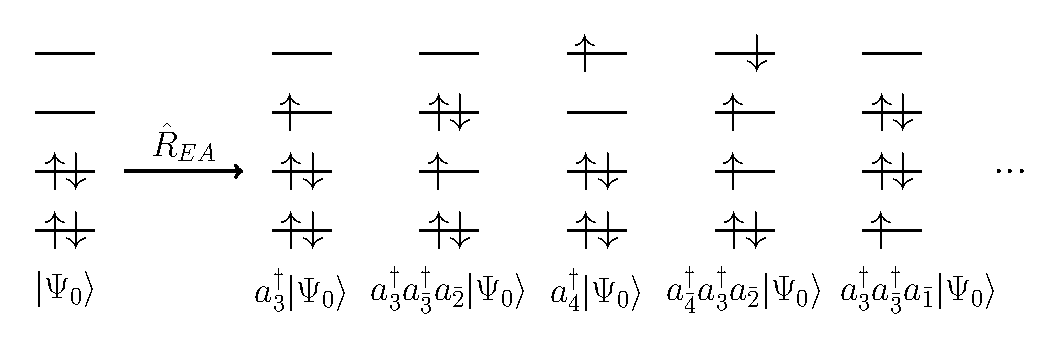
\includegraphics[width=.8\textwidth]{chapters/theory/image/EOM_EA}
    \caption[EOM-EA]{Schematic representation of the EOM-EA method. The target state is generated by applying the electron attachment operator $\hat{R}^{\mathrm{EA}}$ to the reference state. The resulting wavefunction contains contributions from various determinants with one more $\mathrm{\alpha}$ electron.}
    \label{fig:EOM}
\end{figure}

The form of the operator $\hat{R}$ is similar to the cluster operator and chosen to access the desired target state. In the case of EOM-EA, the electron attachment operator $R^{\text{EA}}$ includes terms that describe the creation of one electron in an unoccupied orbital, terms that describe the creation of one electron accompanied by the excitation of another electron:
\begin{equation}\label{eq:R_EA}
    \hat{R}^{\mathrm{EA}} = \hat{R}_1^{\mathrm{EA}} + \hat{R}_2^{\mathrm{EA}} + \ldots = \sum_{a} r^a a_a^{\dagger} + \frac{1}{2}\sum_{ab} \sum_{i} r^{ab}_{i} a_a^{\dagger} a_b^{\dagger} a_i + \ldots
\end{equation}

where $a$ and $b$ denote virtual orbitals, $i$ denotes an occupied orbital, and $r^a$ and $r^{ab}_{i}$ are the coefficients to be determined. By truncating $\hat{R}$ at the same excitation level as the cluster operator, the method is rigorously size-extensive and size-consistent. The EA energies, or any other EOM energy, can be obtained as the eigenvalues of the similarity-transformed Hamiltonian, $\bar{H}_{\mathrm{N}}$:
\begin{equation}
    \bar{H}_{\mathrm{N}} \hat{R} | \Psi_0 \rangle = \Delta E_{\mathrm{EOM}} \hat{R} | \Psi_0 \rangle
\end{equation}
\begin{equation}
    \bar{H}_{\mathrm{N}} = e^{-\hat{T}} \hat{H} e^{\hat{T}} - \langle \Psi_0 | e^{-\hat{T}} \hat{H} e^{\hat{T}} | \Psi_0 \rangle
\end{equation}
As in coupled cluster, the similarity transformed Hamiltonian is non-Hermitian and left and right eigenvectors are different but correspond to the same eigenvalues. This means that the properties have `right' and `left' transition moments. The left deexcitation operator $\hat{L}$, analogous to $\hat{R}$ for the left eigenstates, takes the following form for EOM-EA:

\begin{equation}
\hat{L}^{\mathrm{EA}} = \hat{L}_1^{\mathrm{EA}} + \hat{L}_2^{\mathrm{EA}} + \ldots = \sum_{a} l^i a_a + \frac{1}{2}\sum_{ab} \sum_{i} l^{i}_{ab} a_i^{\dagger} a_b a_a + \ldots
\end{equation}

Where $l_a$ and $l_{ba}^{i}$ are the amplitudes to be determined. And the `left' wavefunction is $\langle\Psi_{\mathrm{EOM}}| = \langle\Psi_{\mathrm{CC}}| \hat{L} = \langle\Phi_0|\hat{L}e^{-\hat{T}}$.

One strength of the EOM-CC ansatz is the ability to use of a closed shell reference to access open shell states, which are eigenfunctions of the $\hat{S}^2$ operator. 
Finally, in the case relevant to this work, the computational cost of the EOM component in EA-EOM-CC methods scales as $\mathcal{O}(N^{5})$, thus rendering the CC reference the computational bottleneck. This is still true in the case of CC2, which also scales as $\mathcal{O}(N^{5})$, since its expression contains more nonlinear terms.

\section{Dyson Orbitals}

Dyson orbitals\cite{jagau2016characterizing,melania2007dyson} are defined as the overlap between the wavefunction of an initial $N$-electron state ($|\Psi_0^N\rangle$) and the wavefunction of the final state with $N\pm1$ electrons ($|\Psi_f^{N+1}\rangle$).
\begin{equation}
    \phi_{d}(r_1) = \sqrt{N} \int \Psi^{N}(r_1,\dots,r_{N-1}) \Psi^{N+1}(r_1, r_2,\dots,r_N)\,dr_1 \dots dr_{N-1}
\end{equation}
Because the terms differ in one electron, the result of the overlap is a scalar field, which is a vector in the Hilbert space, expressed as a linear combination of the molecular orbitals ($\phi_p(r)$) of the reference wavefunction:
\begin{equation}
    \phi_{d}(r) = \sum_p \gamma_p \phi_p(r)
\end{equation}
where $\gamma_p$ are the coefficients that quantify the contribution of each molecular orbital to the Dyson orbital. Physically, Dyson orbitals can be interpreted as the correlated analogue to the orbital of the electron that is either removed or attached. The squared norm of the Dyson orbital, $P$, is calculated by integrating over all space:
\begin{equation}
    P = \int |\phi_{d}(r)|^2 \,dr = \sum_{p,q} \gamma_p^* \gamma_q \langle \phi_p | \phi_q \rangle
\end{equation}
It ranges from 0 to 1 and provides a direct measure of the one-electron character of the ionization or electron attachment process. If the open shell wavefunction is obtained by means of an EOM-CC method, there is a `left' and a `right' Dyson orbital. By convention, the right Dyson orbital is obtained when $\Psi^{N+1}$ is in the bra and $\Psi^{N}$ is in the ket.\\

On top of providing a visual representation of the ionization or electron attachment process, they can be used for the interpretation and prediction of photoelectron spectra as they contain all the information required to calculate differential cross-sections, $\displaystyle{\frac{d\sigma}{d\Omega_k}}$:
\begin{equation}
    \frac{d\sigma}{d\Omega_k} = \frac{4\pi^2kE}{c}|\langle \phi_d | \mu | \Psi^{el}_k \rangle |^2
\end{equation}
where \textit{k} is the magnitude of the photoelectron wavevector, \textit{E} is the energy of the ionizing radiation, and \textit{c} is the speed of light, $\mu$ is the dipole operator, and $\Psi^{el}_k$ is the photoelectron wavefunction, and strong orthonormality is assumed between the reference and continuum wavefunction.  

\subsection{EOM-CC2 Dyson Orbital Equations\label{sec:theory_dyson}}

The algebraic expressions for the EOM-CC2 Dyson orbitals are identical to the CCSD ones. A derivation of the algebraic expression of Dyson orbitals in terms of the $t,\, r,\, l,\, \lambda$ amplitudes is presented for the EA-EOM case, and the expression for the other EOM flavours implemented in this work are provided.\\

It is important to realize that the operators involved ($\hat{T},\hat{\Lambda},\hat{R},\hat{L}$) affect the occupation of the spin-orbitals, and thus only the combinations of terms which leave the reference wavefunction, $| 0 \rangle$, unchanged survive. To find these combinations, commutators can be used to reorder the operators involved. To simplify the equations involved, a change of notation is introduced: $| \Psi_{CC} \rangle \equiv | CC \rangle $ and $| \Psi_{EOM} \rangle \equiv | EOM \rangle $. 

\subsubsection{EOM-EA-CC Dyson Equations}\label{sec:theory_eom_ea_dyson}

In the case of the right EOM-EA-CC Dyson orbital amplitudes:
 \[\gamma^\mathrm{EA,R}_{i} = \langle EA | \hat{a}^{\dagger}_i | CC \rangle =  \langle 0|\hat{L}^{EA} e^{-\hat{T}} \hat{a}^{\dagger}_i e^{\hat{T}} | 0 \rangle \]
 The following equalities are useful:
\[
e^{-{\hat{T}}}e^{{\hat{T}}}=e^{{\hat{T}}}e^{-{\hat{T}}}=1 \]\[
[e^{\pm{\hat{T}}},\hat{a}^{\dagger}_p]=\cancelto{0}{[1,\hat{p}^{\dagger}]} \pm  \sum_{bj} t^b_j[\hat{b}^{\dagger}\hat{j},\hat{p}^{\dagger}] + \sum_{bcjk} \frac{1}{2}t^{bc}_{jk}[\hat{b}^{\dagger}\hat{c}^{\dagger}\hat{j}\hat{k},\hat{p}^{\dagger}] + \ldots
\]
where a change of notation, $a^\dagger_p \rightarrow p^\dagger$, upon expansion is done for readability. Two cases are distinguished, $p$ is a virtual orbital, $a$, or an occupied orbital, $i$.
For virtual orbitals, $p=a$:
\[
[\hat{b}^{\dagger}\hat{j},\hat{a}^{\dagger}] = \hat{b}^{\dagger}\hat{j}\hat{a}^{\dagger} - 
\hat{a}^{\dagger}\hat{b}^{\dagger}\hat{j} = (-1)^2\hat{a}^{\dagger}\hat{b}^{\dagger}\hat{j} - 
\hat{a}^{\dagger}\hat{b}^{\dagger}\hat{j} = 0 \] Similarly with higher order terms, one arrives at:
\[
[e^{\pm {\hat{T}}},\hat{a}^{\dagger}_a] = 0 
\]
For occupied orbitals, $p=i$:
\[
[\hat{b}^{\dagger}\hat{j},\hat{i}^{\dagger}] = \hat{b}^{\dagger}\hat{j}\cancelto{0}{\hat{i}^{\dagger}} - 
\hat{i}^{\dagger}\hat{b}^{\dagger}\hat{j} \] And similarly with higher order terms:
\[
[e^{\pm {\hat{T}}},\hat{a}^{\dagger}_i] = -\hat{a}^{\dagger}_i(e^{\pm {\hat{T}}}-1) 
\]
These relations can now be used to derive the expression for the occupied and virtual right EOM-EA-CC Dyson orbital amplitudes: \[ \phi^\mathrm{EA,R}_\mathrm{D} = \sum_p^\mathrm{} \gamma^\mathrm{EA,R}_p \phi_p= \sum_i^\mathrm{occ} \gamma^\mathrm{EA,R}_i \phi_i + \sum_a^\mathrm{vir} \gamma^\mathrm{EA,R}_a \phi_a \]
The general expression can be reordered:
\noindent\begin{flalign}
   \gamma^\mathrm{EA,R}_{p} &= \langle EA | \hat{a}^{\dagger}_p | CC \rangle =  \langle 0|\hat{L}^{EA}e^{-{\hat{T}}}\hat{a}^{\dagger}_p e^{\hat{T}} | 0 \rangle \notag \\
    &= \langle 0|\hat{L}^{EA}(\hat{a}^{\dagger}_p e^{-{\hat{T}}} + [e^{-{\hat{T}}},\hat{a}^{\dagger}_p]) e^{\hat{T}} | 0 \rangle
\end{flalign}
For virtual orbitals, $p=a$:
\noindent\begin{flalign}
    \gamma^\mathrm{EA,R}_{a} &= \langle 0|\hat{L}^{EA}(\hat{a}^{\dagger}_a e^{-{\hat{T}}} + \cancelto{0}{[e^{-{\hat{T}}},\hat{a}^{\dagger}_a]}) e^{\hat{T}} | 0 \rangle \notag \\
    & = \langle 0|\hat{L}^{EA}\hat{a}^{\dagger}_a\, \cancelto{1}{e^{-{\hat{T}}}e^{\hat{T}}} | 0 \rangle = \langle 0|\hat{L}^{EA}\hat{a}^{\dagger}_a | 0 \rangle \notag \\
    & = \langle 0| l_a \hat{a} \hat{a}^\dagger | 0 \rangle \notag \\
    & = l_a
\end{flalign}
For occupied orbitals, $p=i$:
\noindent\begin{flalign}
    \gamma^\mathrm{EA,R}_{i} &= \langle 0|\hat{L}^{EA}(\hat{a}^{\dagger}_i e^{-{\hat{T}}} + [e^{-{\hat{T}}},\hat{a}^{\dagger}_i]) e^{\hat{T}} | 0 \rangle \notag \\
    & = \langle 0 | \hat{L}^{EA}(\cancelto{0}{\hat{a}^{\dagger}_i e^{-{\hat{T}}} -\hat{a}^{\dagger}_ie^{-{\hat{T}}}} + \hat{a}^{\dagger}) e^{\hat{T}} | 0 \rangle = \langle 0 | \hat{L}^{EA} \hat{a}^{\dagger}_i e^{\hat{T}} | 0 \rangle  \notag \\
    & = \langle 0 | \sum_b l_b t_i^b \, \hat{b} \hat{i}^{\dagger} \hat{b}^{\dagger}\hat{i}+ \frac{1}{2} \sum_{jbc} l_{bc}^j t_{ij}^{bc} \, \hat{b}\hat{c}\hat{j}^{\dagger}\hat{i}^{\dagger}\hat{b}^{\dagger}\hat{c}^{\dagger}\hat{i}\hat{j} | 0 \rangle  \notag \\ 
    &  = - \sum_b t_{ib} l_b - \frac{1}{2} \sum_{jbc} t_{ji}^{bc} l_{bc}^k
\end{flalign}
A similar approach can be applied to the other Dyson equations to obtain their corresponding expressions, which can be found in appendix \ref{ch:appendix:dyson}.

%%%%%%%%%%%%%%%%%%%%%%%%%%%%%%%%%%%%%%%%%%%%%%%%%%
% Keep the following \cleardoublepage at the end of this file, 
% otherwise \includeonly includes empty pages.
\cleardoublepage

% vim: tw=70 nocindent expandtab foldmethod=marker foldmarker={{{}{,}{}}}